% Chapter 1

\chapter{Data Set} % Main chapter title

\label{Chapter3} % For referencing the chapter elsewhere,  use \ref{Chapter1}
\lhead{Chapter 3. \emph{Data Set}} % This is for the header on each page - perhaps a shortened title
%----------------------------------------------------------------------------------------
\emph{The social network meta data related to images can be used for
image classification tasks and some times can outperform image
content based methods.} For the validation of this
hypothesis, we needed a well labeled image data set, which should also
be amenable to expansion along social dimensions.
The data must have some ground truth provided by human annotators or
by some other standard way of labeling.

Most of the Large Scale Image Benchmarks are usually assembled by
using the vast number of images available on the web. These images
are  mostly part of social media holders like Pin-interest,
Flickr and Facebook. After exploring the available image benchmarks,
we narrowed our focus to the following four well established
benchmarks, because these were created from Flickr images and by
implementing the Flickr APIs on available information, we could
extract enough social meta data about these images:
\begin{itemize}
\item The PASCAL Visual Object Challenge ('PASCAL') \cite{PASCAL}
\item The MIR Flickr Retrieval Evaluation ('MIR') \cite{MIR}
\item The ImageCLEF Annotation Task ('CLEF') \cite{CLEF}
\item The NUS Web Image Database ('NUS') \cite{NUS}
\end{itemize}
The creators of these data sets had obtained labels through
crowdsourcing from the Flickr users  or communities. The labels
ranged from object based categories like \textit{person} or \textit{bicycle}, to
subjective concepts like \textit{Aesthetic\_ Impression}. These
labels satisfied the desired ground truth constraint for our
classification process. We, therefore, used these labels as a
classification base for our analysis.

\section{Description of Data sets}
The PASCAL Visual Object Challenge ('PASCAL') consists of over
12,000 images collected since 2007, with additional images added
each year. Flickr sources were available only for
training images, and for the test images from 2007. There were a total
of 11,197 images, for which Flickr sources were available.

The MIR Flickr Retrieval Evaluation ('MIR') consists of
one million images, 25,000 of which have been annotated. Flickr
sources were available for 15,203 of the annotated images.

The ImageCLEF Annotation Task ('CLEF') uses a subset of
18,000 images from the MIR data set, but it has more varied tagging
as annotation. There were a total of 4,807 images, for which Flickr
sources were available.

The NUS Web Image Database ('NUS') consists of
approximately 270,000 Images. Flickr sources were available for all
images.
\section{Augmentation of Social Meta-data}
Flickr Sources of above data sets were provided by the data set
creators. We used the possible Flickr APIs and tried to obtain the
maximum meta data for each photo instance. The information, we could
extract were:
\begin{itemize}
\item 	The photo itself
\item 	Photo data,
\begin{itemize}
\item Title
\item Description
\item Location
\item Time stamp
\item View count
\item Upload date
\end{itemize}
\item 	User information, including the uploader's name, username, location, their network of contacts, etc.
\item 	Photo tags, and the user who provided each tag
\item 	Groups to which the image was submitted
\item 	Collections (or sets) in which the photo was included
\item 	Galleries in which the photo was included
\item 	 Comment threads for each image instance
\end{itemize}
We considered only the images which have all the above data available,
which is roughly 90\% of the images for which the URL Source was available.
\section{Preliminary Observation of Data set}
We also made some observations while extracting the data. We would like to
give those observations at this stage because it will help us
describe the inferences and results.
\begin{center}
\begin{figure}
\centering
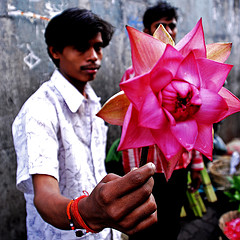
\includegraphics[width=3cm, height=3cm]{./Pictures/MIR/1.jpg}
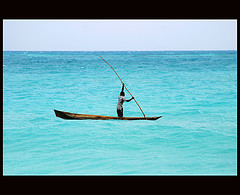
\includegraphics[width=3cm, height=3cm]{./Pictures/MIR/2.jpg}
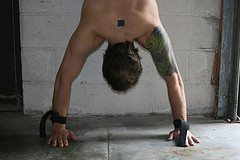
\includegraphics[width=3cm, height=3cm]{./Pictures/MIR/3.jpg} \\
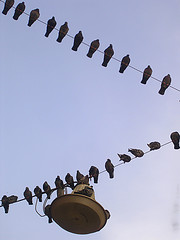
\includegraphics[width=3cm, height=3cm]{./Pictures/MIR/4.jpg}
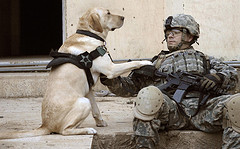
\includegraphics[width=3cm, height=3cm]{./Pictures/MIR/5.jpg}
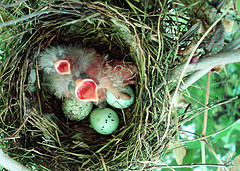
\includegraphics[width=3cm, height=3cm]{./Pictures/MIR/6.jpg}
\caption{Image MIR Examples}
\label{fig:Image MIR Examples}
\end{figure}
\end{center}
\vspace*{1cm}
\begin{center}
\begin{figure}
\centering
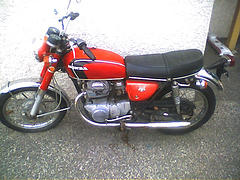
\includegraphics[width=3cm, height=3cm]{./Pictures/PASCAL/1.jpg}
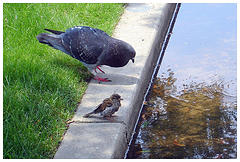
\includegraphics[width=3cm, height=3cm]{./Pictures/PASCAL/2.jpg}
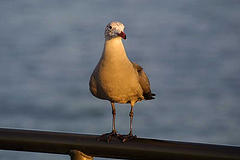
\includegraphics[width=3cm, height=3cm]{./Pictures/PASCAL/3.jpg} \\
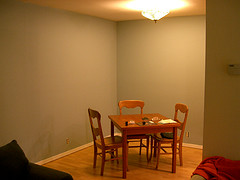
\includegraphics[width=3cm, height=3cm]{./Pictures/PASCAL/4.jpg}
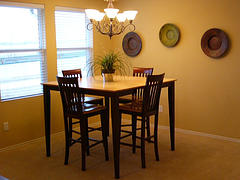
\includegraphics[width=3cm, height=3cm]{./Pictures/PASCAL/5.jpg}
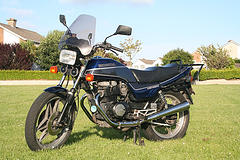
\includegraphics[width=3cm, height=3cm]{./Pictures/PASCAL/6.jpg}
\caption{Image PASCAL Examples}
\label{fig:Image PASCAL Examples}
\end{figure}
\end{center}
The statistics obtained from enriching the images and elementary
statistical analysis of image properties reveals that there is a
large difference between the data-sets. For example, PASCAL had the least
tags and comments compared to all other data-sets, because it was made
up of less interesting images. The NUS data set favored the highly
popular images and we saw that it has the highest tag vs image
ratio of 19.4. The images were highly tagged, had large number of
comments and were submitted to many groups. The MIR had 17$+$ tags
and comments showing that it also had some what interesting images.

%\[Attach some SCATTER PLOTS if you need\]\\
\begin{center}
\begin{figure}
\centering
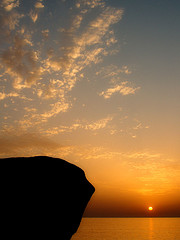
\includegraphics[width=3cm, height=3cm]{./Pictures/CLEF/1.jpg}
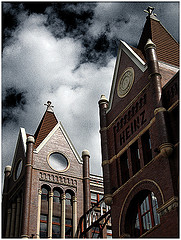
\includegraphics[width=3cm, height=3cm]{./Pictures/CLEF/2.jpg}
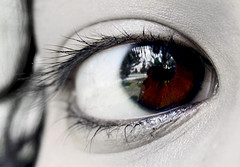
\includegraphics[width=3cm, height=3cm]{./Pictures/CLEF/3.jpg} \\
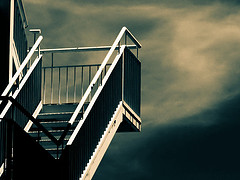
\includegraphics[width=3cm, height=3cm]{./Pictures/CLEF/4.jpg}
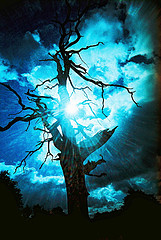
\includegraphics[width=3cm, height=3cm]{./Pictures/CLEF/5.jpg}
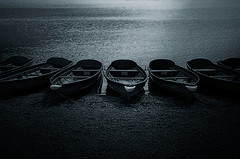
\includegraphics[width=3cm, height=3cm]{./Pictures/CLEF/6.jpg}
\caption{Image CLEF Examples}
\label{fig:Image CLEF Examples}
\end{figure}
\end{center}
\vspace*{1cm}
\begin{center}
\begin{figure}
\centering
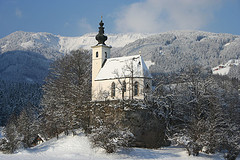
\includegraphics[width=3cm, height=3cm]{./Pictures/NUS/1.jpg}
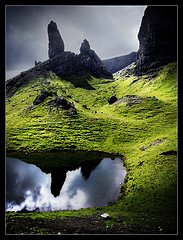
\includegraphics[width=3cm, height=3cm]{./Pictures/NUS/2.jpg}
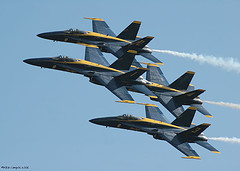
\includegraphics[width=3cm, height=3cm]{./Pictures/NUS/3.jpg} \\
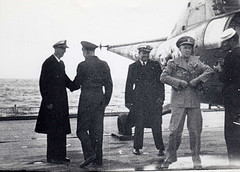
\includegraphics[width=3cm, height=3cm]{./Pictures/NUS/4.jpg}
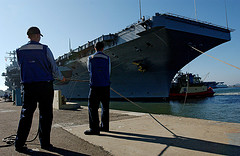
\includegraphics[width=3cm, height=3cm]{./Pictures/NUS/5.jpg}
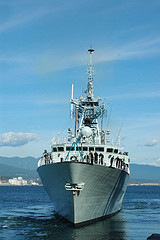
\includegraphics[width=3cm, height=3cm]{./Pictures/NUS/6.jpg}
\caption{Image NUS Examples}
\label{fig:Image NUS Examples}
\end{figure}
\end{center}
\vspace*{1cm}
\section{Label Selection for Classification Problem}
Due to constraints of less number of images for some particular labels and balanced learning, we have to selectively
choose the labels for our Classification Problem.

For example, CLEF has 99 labels and some labels have number of images less than even 17. Doing learning and testing on such a small set was not useful and would not have given good results. We, therefore, in case of CLEF selected 20 Labels which had sufficient data.

Similarly for NUS, because of some computational constraints and data availability, we reduce our computation to 12 labels. The following table shows the labels, which were considered for the whole classification problem.

%-------------------- Table example ------------------------------
\begin{table}[ht]
\caption{Labels} % title of Table
\centering % used for centering table
\begin{tabular}{|c|p{2cm}|p{7cm}| } % centered columns (4 columns)
\hline\hline %inserts double horizontal lines
Data set & Count of Labels & Selected Labels \\ [0.5ex] \hline% inserts table
%heading
\hline % inserts single horizontal line
NUS & 10 & animal, coral, dancing, harbor, military, mountain, snow, statue, tattoo, temple, waterfall, wedding \\  [1ex] \hline
PASCAL & 20 & aeroplane, bicycle, bird, boat, bottle, bus, car, cat, chair, cow, dining table, dog, horse, motorbike, person, potted plant, sheep, sofa, train, tv monitor \\  [1ex] \hline
MIR & 14 & flower, car, bird, dog, night, tree, clouds, portrait, female, male, people, sea, river, baby \\  [1ex] \hline
ImageCLEF & 20 & Adult, Aesthetic Impression, Animals, Autumn, Citylife, cute, Day, Flowers, Food, Graffiti, Landscape\_ Nature, Painting, Portrait, Single Person, Sky, Street, Summer, Sunset Sunrise, Vehicle, Winter \\  [1ex] \hline
\hline %inserts single line
\end{tabular}
\label{table:nonlin} % is used to refer this table in the text
\end{table}
%--------------------- end of the example ------------------------
Following the ideas give in \citet*{Jure}, we decided to construct the whole problem of labeling an image with multiple label as taking a single label and then decide, if that image should or should not be given that label.

We, therefore, supposed to learn a prediction for an image $x_n$ and label $l$, which will be $\bar{y_l} (x_n,\theta_l)\in\{-1,1\}$.  $\theta^l$ are the descriptors/features extracted for label $l$. The above strategy transformed the whole problem in multiple binary classification problem. We followed the following strategy:

  Given an image data set consisting of N images $X = \{x_1 ...x_N\}$ and a label space consisting of L categories $L = \{-1, 1\}^L$. We take single label  $l$,  when we combine the ground truth for the entire data set for label $l$, we get $y^n_l \in \{-1,1\}^N$. Now we learn a classifier, which predicts for an image $x_n$ as $\bar{y_l} (x_n,\theta^l)\in\{-1,1\} $. $\theta^l$ are  descriptors/features extracted for label $l$.

	 This gave us good learning of features for each label and also precise information retrieval against a label, because if we use such classifier for a label $l$, we can easily retrieve images for that label by predicting $\bar{y_l} (x,\theta^l)\in\{-1,1\}$ for set of images.
	
	 It also gave a leverage of easily using the bag of visual/non-visual words. Bagging of visual/non-visual words means we tried to learn some small set of descriptors, called as words, which represent a category.

%-----{\bf *** The above paragraph is totally confusing. I cannot understand
%what you are trying to say. What kind of binary classification are you
%doing 1 vs rest or 1 vs 1. How will you give the final set of labels?
%What do you mean by bag of visual/non-visual words? What do you mean
%by bagging here? You have to rewrite the whole para and explain what
%you mean more precisely. ***}

\section{Comparison of Results}
%{\bf *** Some where you have to say what is your baseline. What will you
%compare your results to? ***}

In next two chapter, we would be first using the visual descriptors to classify images for each label. After that, we would be using social meta-data for image classification. We  would be comparing these two results to figure out, which works out best among these two. These all tasks will be done for each label individually.
In subsequent part, we will be doing ensemble of these classifiers to leverage all the descriptors. We will also show comparisons with published results on each of these four benchmarks or with results in associated competitions. All these benchmarks has their own competition and also various authors used these benchmarks in their paper, which we will be using.. In \citet*{MIRresults}, \citet*{CLEF} ,\citet*{PASCAL} and  \citet*{NUS}, authors have either surveyed the various results in competition or have depicted a way of using visual + social data as classification basis for MIR, ImageCLEF, PASCAL and NUS respectively. We will consider results from these papers. We will also be giving qualitative and quantitative conclusions/observations  of our results.

The goal of all these comparisons would be to assess the improvement that was obtained by using social meta-data for images. We reported the mean average precision (MAP) for the sake of comparison with published materials and competition results. We also gave the accuracy for the binary prediction/classification of labels.


